% !TeX encoding = UTF-8
% !TeX spellcheck = es_ES
% !TeX root = WhatIs.tex
%!TEX root=WhatIs.tex

\documentclass[spanish]{DccDiyTools/DccDiyTools}
\usepackage[spanish]{babel}
\usepackage[
type={CC},
modifier={by-sa},
version={4.0},
]{doclicense}

\usepackage[]{DccDiyTools/DccDiyToolsPics}
\usepackage[]{DccDiyTools/DccDiyToolsComponentTables}


\title{What Is DCC DiY Tools}
\subtitle{Manifiesto de DCC DiY Tools}
\author{Daniel Vilas}
\date{Julio 2022}

\dbHeaderTitle{What Is DCC DiY Tools}
\dbType{M}
\dbDate{22}
\dbCode{002}
\dbStatus{Draft}
\dbVersion{0.1}
%\tikzset{
    pics/SmallBoard/.style={
      code = {
        % \draw [step=0.1,very thin, yellow] (-2,-1) grid (2,1);
        % \draw [step=0.5,very thin, red] (-2,-1) grid (2,1);
        % \draw [very thin, green] (-2,-1) grid (2,1);
        \node[inner sep=0pt] at (0,0)
        {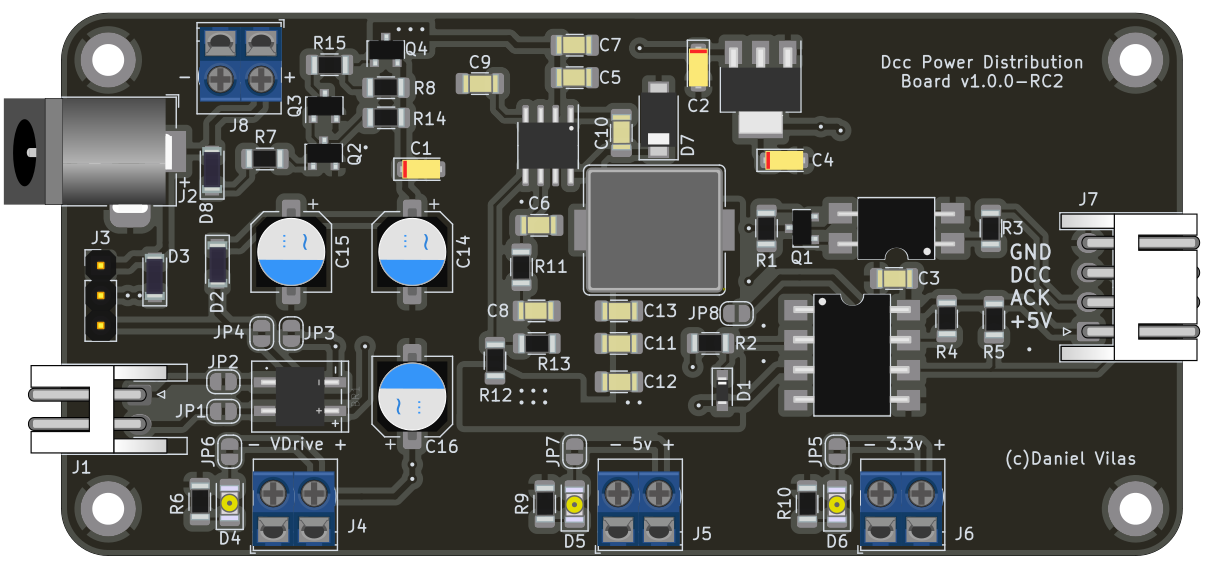
\includegraphics[scale=0.25]{images/front.png}};  


        \node[](-jack) at (-1.35,0.278) {};
        \node[](-terminal) at (-.8,0.65) {};
    }}
}

\tikzset{
    pics/WallAc/.style={
      code = {
    \begin{scope}[shift={(0.25,0)}]
        % \draw [step=0.1,very thin, yellow] (-2,-2) grid (2,2);
        % \draw [step=0.5,very thin, red] (-2,-2) grid (2,2);
        % \draw [very thin, green] (-2,-2) grid (2,2);
        % Mains lead
        \draw[line width=2pt,cap=round, lightgray] (0.05,-0.21) -- (0.05,-0.45);
        \draw[line width=2pt,cap=round, lightgray] (0.275,-0.21) -- (0.275,-0.45);
        % Relief and out cable
        \draw[line width=2pt,cap=round] (-0.5,0.25) -- (-1,0.25);
        \draw[line width=2pt,cap=round,black!75] (-0.55,0.35)--(-0.55,0.15);
        \draw[line width=2pt,cap=round,black!75] (-0.63,0.325)--(-0.63,0.175);
        \draw[line width=2pt,cap=round,black!75] (-0.71,0.3)--(-0.71,0.2);
        \draw[line width=2pt,cap=round,black!75] (-0.79,0.275)--(-0.79,0.225);
        \draw[line width=2pt,cap=round,black!75] (-0.87,0.275)--(-0.87,0.225);

        \draw[line width=2pt,rounded corners=1pt,fill=black!75] (-0.5,0) rectangle +(1,0.5);
        \draw[line width=2pt,rounded corners=1pt,fill=black!65] (-0.1,0) rectangle +(0.5,-0.2);
        % \draw[line width=2pt,cap=round, gray] (0.05,-0.21) -- (0.05,-0.45);
        % \draw[line width=2pt,cap=round,gray] (0.275,-0.21) -- (0.275,-0.45);

        \node[white,scale=0.5] at (0,0.25) {DC Wall};
        \node[](-jack) at (-1.1,0.25) {};
        \node[](-mains) at (.1625,-0.55) {};
    \end{scope}
    }}
}

\begin{document}
\maketitle
\newpage
\section{Introduccion}
% !TeX encoding = UTF-8
% !TeX spellcheck = es_ES
% !TeX root = CBus.tex
%!TEX root=CBus.tex
C-Bus es un standard LCB usado y promocionado por MERG\copyright. A bajo nivel utiliza un Bus CAN como transporte fisico de datos entre modulos (electronicos).

La idea de despligue es usar una topolgia de bus:
\begin{figure}[H]
    \centering
    \begin{tikzpicture}
        %\draw [very thin, green]  (-6,-3) grid (6,3);
        \node at (-6,3) [rectangle,draw,align=left] (ps) {Previous\\Segment};
        \node at (6,3) [rectangle,draw,align=left] (ns) {Next\\Segment};
        
        \node at (-2.75,0) [rectangle,draw,align=left] (d1) {Modulo 1};
        \node at (0,0) [rectangle,draw,align=left] (d2) {Modulo 2};
        \node at (2.75,0) [rectangle,draw,align=left] (d3) {Modulo ...};

        \draw [line width=2, blue] (-4,3) -- (-4,0) --(d1.west);
        \draw [line width=2, blue] (-1.25,3) -- (-1.25,0) --(d2.west);
        \draw [line width=2, blue] (1.5,3) -- (1.5,0) --(d3.west);

        \draw [line width=5] (ps.east) -- (ns.west);
    \end{tikzpicture}
    \caption{C-Bus Segmento}
    \label{fig:cBusSegment}
\end{figure}

Al final de un segmento puede haber otro segmento, un repetidor, un convertidor a Ethernet,\dots.
Desde el bus a los dispositivos es necesario tener un latiguillo.




\newpage
\section{¿Que es?}
% !TeX encoding = UTF-8
% !TeX spellcheck = es_ES
% !TeX root = WhatIs.tex
%!TEX root=WhatIs.tex

En un principio, como la mayoria de los aficionados al tren en miniatura, la aventura empieza hace unos años con un ovalo de vias,
un transformador o mando analogico, una maquina y un par de vagones. El sistema digital DCC ya existe pero aun compite con otros\sidenote{Como "delta", MFX,\dots},
y aun no es muy accesible en terminos economicos. A su vez acaba de aparecer la platafoma de microntroladores Arduino que permite,
entre otras cosas, generar una señal PWM para controlar motores.

Armados con un con Arduino UNO, un Motor-Shield y un adapatador de corriente continua unos valientes comprueban que es posible
controlar la velocidad de un tren y su direccion digitalmente. A partir de esto ellos mismos se fabrican unos circuitos sencillos
para dar algo más de funcionalidad, como una placa que usa la corriente de accesorios del transformador analogico, un display
LCD de 20x02 caracteres, una placa de proteccion ante corto circuitos,\dots

Con el tiempo el sistema DCC se hace más accesible, y ademas, la lista de modulos creados se amplia a cosas DCC, y a su vez los estos son más
genericos y reutilizables\sidenote{Sin o con pocas modificaciones}. Han pasado de ser algo muy particular para los problemas de
una maqueta, a ser herramientas que puden ser usadas en todas las maquetas.

En un momento dado se da la posibilidad de hacer una nueva maqueta y se toma la decision de normalizar\sidenote{O standarizar,
como se prefiera decir} una serie de componentes(Conectores, cables, etc\dots) y con ella de documentar los modulos que se hagan
como si fuera un producto comercial. Ha nacido DCC DiY Tools.
\begin{itemize}
    \item \textit{DCC DiY Tools} es una declaracion de intenciones. De la intencion de hacer las cosas bien.
    \item Hacer los modulos reutilizables y adaptables a cualquier maqueta, como un producto de una empresa
    \item Con calidad y repetibilidad. Pudiendo garantizar que se cumplen las especificaciones. 
    \item Siguiendo una normativa propia, como por ejemplo de conectores, para que los modulos sean similares
    \item Con los documentos necesarios equivalentes a los que se necesitan en una empresa, tales como manuales de usuario, de 
    analisis y diseño, esquematicos, \dots
    \item Basado en la descripcion de Open Source HardWare, o OSHW, con toda la documentacion abierta y libre. Ya no solo la 
    minima requerida por la OSHW, si no de las decisiones tomadas y su razon.
    \item Seran educativos. O que puedan servir\sidenote{Aunque sea de lo que no hay que hacer} para entender las cosas.
    \item Un conjunto de repositorios git o similar.
\end{itemize}

En resumen \textit{Dcc DiY Tools} es un repositorio de informacion abierta, lo mas completa posible, de modulos OSHW usables
en maquetas de tren, tanto digitales, como analogicas.

Al ser más inforamacion que otra cosa, la licencia y la garantia de los productos manufacturados es la definida por OSHW, 
que se puede resumir\sidenote{Mas mal que bien} en  "<haz lo que quieras, sin ninguna garantia">, ver el apartado de
garantia y licencia para una informacion detallada.

\subsection{¿Que no es?}
DCC DiY Tools \textbf{no} es una empresa, ni una linea de productos, ni una tienda ni nada mas que un sitio de documentacion. 
Tampoco es un sitio web con una comunidad\sidenote{Ojala se convierta en ello.} que pueda dar soporte rapido\sidenote{Mientras
 tanto se dara lo que se pueda}.
En realidad es una persona intentando documentar sus circuitos de tal forma que les puedan servir a otros.

\newpage
\section{Modulos DCC DiY Tools}
% !TeX encoding = UTF-8
% !TeX spellcheck = es_ES
% !TeX root = WhatIs.tex
%!TEX root=WhatIs.tex
\textit{DCC DiY Tools} como se ha dicho es un repositorio de informacion sobre
modulos para usar en maquetas de tren y similares, y los tipos de modulos que tiene
bajo su paraguas son de varios tipos, segun sus "<artefactos generados">. Principalmente
son tres tipos:
\begin{itemize}
    \item \textbf{Documentacion}: El resultado solo es uno o varios documentos
    \item \textbf{Modulo Electronico}: Se tendra la documentacion y los ficheros necesarios 
    para poder adquirir y fabricar una placa de circuito impreso. 
    \item \textbf{Objeto Imprimible 3D}: Lo mismos que el anterior, pero para poder 
    imprimir un objeto 3d.
\end{itemize}

Todos los modulos tendran un identificador "<\textbf{AA-SSS}"> dode "<AA"> son las dos
ultimas cifras del año actual y "<SSS"> un número secuencial. A partir de este identificador
se pueden generar idenficadores para cada artefacto.

Los artefactos se identificaran con el esquema "<\textbf{T AA-SSS[-N]}">, donde "<T"> es una
letra que identifica el tipo y "<N"> un número secuencial, empenzando en 1 para el primer
artefacto. Este numero se añadira en el caso de que el modulo se componga de varios
artefactos.

Para que un modulo sea Dcc DiY Tools, es necesario que cumplan las normativas que se
definan en los documentos/modulos correspondientes. Estos documentos contendran 
normas obligatorias, como formatos y otros más laxos como recomendaciones.

Todos los modulos deberan estar publicados bajo una licencia libre, como Creative-Commons,
OSHW, o cualquier otra similar. Y ademas con todos los artefactos necesarios para poder
fabricar o manufacturar el objeto fisico. 

\newpage
\section{Adquirir modulos DCC DiY Tools}
% !TeX encoding = UTF-8
% !TeX spellcheck = es_ES
% !TeX root = WhatIs.tex
%!TEX root=WhatIs.tex
Los modulos \textit{DCC DiY Tools} no tienen una tienda oficial, por lo que no
se pueden comprar directamente de la iniciativa actual. Pero, como es un requisito que
todos los modulos esten bajo una licencia libre y conentengan los artefactos necesarios
para su manufactura, cualquiera puede solicitar su fabricacion a una empresa
especializada\sidenote{O hacerlo en su casa si sabe como\dots}.

\subsection{Compra Conjunta}
Para un ahorro de costes se recomienda hacer una compra conjunta por parte de algun
colectivos, como una asociacion de modelismo, foro o similar. Los fabricantes de 
PCBs suelen tener un minimo de placas a pedir\sidenote{Que puede ser pequeño, 5, o 
grande, 100}, por lo que para un individal puede subir mucho el precio para 
una sola placa.

Recordemos que por muy seria que sea la fabrica de PCBs y el origen de los componentes
siempre debemos esperar fallos de calidad\sidenote{O fallos por nuestra parte} y
necesitaremos unos cuantos extras para aseguranos que hay suficientes modulos fabricados
para todos los interesados.

\subsection{Artefactos Documentos}
Estos artefactos por normativa seran PDF con licencia \doclicenseName por lo que 
cualquiera tiene permitido imprimir las copias que necesite, incluso maquetar un libro
y venderlo. 
Las fuentes estaran disponibles en formato \LaTeX, o en su defecto ODT. para que 
cualquiera tambien pueda ajustarlo a sus necesidades.

En la seccion de licencia podras encontrar más informacion al respecto.

En el caso de no querer imprimir muchas paginas, recomendamos contactar con alguna
imprenta, o copisteria, para conseguir un precio más economico. O incluir una pagina
con los QR para acceder a la version en GitHub del documento correspondiente.

\subsection{Artefactos PCB}
El caso de los artefactos que sean placas de circuito impreso en el repositorio Git 
se incluira un fichero ZIP con los gerber necesarios para enviar a un fabricante low
cost en china\sidenote{En estos momentos JLCPCB, pudiendo variar en el tiempo}, asi
como los ficheros de proyecto en un EDA OpenSource\sidenote{KiCad}.

Tambien se acompañara con un xls con el listado de materiales necesarios y donde sea
posible los ficheros extra para PCBA del mismo fabricante low cost.

En general realizar un pedido solo requerira enviar dicho zip utilizando un formulario
y validar las dimensiones junto la posicion de los taladros. En el caso de que se 
necesitara algo especifico se documentaria para dicho artefacto.

\subsection{Artefactos 3D}
Para los artefactos que sean objetos 3D se incluiran los ficheros
correspondientes de un modelador 3D open source como FreeCad, Blender, o Fusion360
\footnote{Lo consideramos como OpenSource por que para proyectos OSS la licencia es 
gratis y es un standard de facto} y los ficheros STL\sidenote{U otros similares}, 
que permitan ser impresos en una impresora 3D "<casera"> o enviados a una fabrica
low cost en china.

Al igual que con los artefactos PCB se incluira documentacion en el caso de ser
necesario.

\newpage
\section{Licencia}
% !TeX encoding = UTF-8
% !TeX spellcheck = es_ES
% !TeX root = DccPowerDistribution.tex

La gama de dispositivos DccDiyTools estan bajo una licencia OSHW, que se define como:

"<Hardware de Fuentes Abiertas (OSHW en inglés) es aquel hardware cuyo diseño se hace disponible
públicamente para que cualquier persona lo pueda estudiar, modificar, distribuir, materializar
y vender, tanto el original como otros objetos basados en ese diseño. Las fuentes del hardware
(entendidas como los ficheros fuente) habrán de estar disponibles en un formato apropiado para
poder realizar modificaciones sobre ellas. Idealmente, el hardware de fuentes abiertas utiliza
componentes y materiales de alta disponibilidad, procesos estandarizados, infraestructuras abiertas,
contenidos sin restricciones, y herramientas de fuentes abiertas de cara a maximizar la habilidad
de los individuos para materializar y usar el hardware. El hardware de fuentes abiertas da libertad
de controlar la tecnología y al mismo tiempo compartir conocimientos y estimular la comercialización
por medio del intercambio abierto de diseños.">
\href{https://www.oshwa.org/definition/spanish/}{Extracto de la licencia por OSHWA}

\subsection{Licencia Resumida}
La licencia completa se puede obtener de \href{https://www.oshwa.org/definition/spanish/}{Open Source
Hardware Association - (OSHWA)} pero en resumidas cuentas significa que:
\begin{itemize}
    \item Cualquier persona pueda fabricar, modificar, distribuir y usar esos objetos.
    \begin{itemize}
        \item Quien lo haga tiene la oblicacion de indicar que su producto no ha sido
manufacturado, vendido, garantizado o autorizado en cualquier forma por el diseñador original.
        \item Tampoco puede usar ninguna marca registrada del diseñador original.
    \end{itemize}
    \item Se tiene acceso a la documentacion libremente de por no más que un razonable coste de reproducción.
    \begin{itemize}
        \item La documentacion, se refiere principalmente a los documentos CAD necesarios para manufacturar
        el producto.
        \item Debe estar en un formato facilmente modificable
    \end{itemize}
    \item El software necesario\sidenote[][]{Firmware, software de control,...} debe ser libre o bien
    documentado para que cualquiera pueda crearlo.
    \item Cualquiera persona puede crear obras derivadas y redistirbuir (incluyendo venta) con la misma licencia
de la obra original
    \begin{itemize}
        \item No se deberia requerir el pago de licencias, regalias o similares por la venta.
        \item El diseñador original puede exigir la atribucion de autoria y restringir el nombre en las obras
derivadas.
    \end{itemize}
    \item Cualquiera significa Cualquiera. Sin discriminacion de raza, sexo,... ni discriminacion de ambito
de aplicacion. Nadie debe requerir de una licencia especial para disfrutar de los derechos aqui defenidos.
    \item No se puede restringir otros productos que se distribuyan junto al producto licenciado. 

\end{itemize}

En resumen "<Cualquier persona pueda fabricar, modificar, distribuir y usar esos objetos."> y el diseñador 
puede añadir alguna pequeña restriccion.

\subsection{Licencia DccPowerDistribution}
DccPowerDistribution se licencia mediante la definicion publicada por la \href{https://www.oshwa.org/definition/spanish/}{OSHWA}
con las siguientes consideraciones:
\begin{itemize}
    \item Toda la documentacion y ficheros se encuentra en repositorios publicos de github.
    \begin{itemize}
        \item \url{https://github.com/danielvilas/DigitalTrains/tree/master/DccBlocks/DccPowerDistribution/board}
        \item \url{https://github.com/danielvilas/DigitalTrainsDocs/tree/main/DccDiyTools/DccPowerDistribution} 
    \end{itemize}
    \item Esta licencia OSHW se aplica para la placa electronica DccPowerDistribution 
    \item Los documentos anexos, como manuales, read me y similares, estan bajo la licencia Creative Commons By Share-Alike 
    \ccbysa
    \item Para editar la placa es necesario usar KiCAD 6.0.6 o superior. La documentacion se encentra en \LaTeX
    \item Cualquier placa derivada debe cambiar el nombre lo suficiente como para que sepa que es una placa derivada
    \begin{itemize}
        \item Cambiar el numero de version \textbf{no} es suficiente
        \item Seria valido añadir un nombre corto ([Nombre]DccPowerDistribution o DccPowerDistribution[Nombre]) 
    \end{itemize}
    \item Cualquiera puede manufacturar esta placa y venderla, sin pago de licencias ni regalias al diseñador.
Pero considera hacer una donacion al diseñador, sobre todo en el caso de venta y teniendo un beneficio economico
considerable. 
\end{itemize}

\newpage
\section{Garantia y Consideraciones de Seguridad}
% !TeX encoding = UTF-8
% !TeX spellcheck = es_ES
% !TeX root = WhatIs.tex
%!TEX root=WhatIs.tex
\textit{DCC DiY Tools} no manufactura productos por lo que no proporciona ningun
tipo de garantia legal sobre ningun objecto manufacturado tal como dice la Introduccion
de la licencia OSHW. Es responsabilidad de quien manufacture el modulo soportar
la garantia a los usuarios finales.

Tambien es responsabilidad de quien manufacture asegurarse que no hay fallos de diseño,
y en el caso de encontrarlo notificar a \textit{DCC DiY Tools} del mismo.

Por otra parte \textit{DCC DiY Tools} se asegurara de que:
\begin{itemize}
    \item Usando los materiales del BOM y los procedimiendos descritos, el modulo
    cumple las especificaciones.
    \item El sistema no es peligroso siguendo las indicaciones de seguridad
    \item No hay fallos de diseño conscientes
    \item En la medida de lo posible\sidenote{Y que tenga sentido}, se siguen buenas practicas de diseño:
    \begin{itemize}
        \item Disipacion termica, tamaño de trazas,\dots
        \item Teniendo en cuenta EMI/EMC
        \item Con idea a poder Certificarlo FCC/CE
    \end{itemize}
    \item El diseño se ha probado siguiendo las especificaciones y un pequeño margen extra
\end{itemize}
 
Cada modulo fisico debera contar con su apartado de garantia y consideraciones
de seguridad a partir de este apartado. 

Los modulos \textit{DCC DiY Tools} se espera ser utilizado con sentido comun y se
debe evitar realizar acciones que puedan deriviar en situaciones peligrosas:
\begin{itemize}
    \item No exponer a fuentes de calor que puedan estropear los dispositivo
    \item Las placas electronicas pueden disipar energia en forma de calor, no
    teneras cerca de materiales inflamables y no tocarlas cuando esten en funcionamiento
    \item Situarla en un lugar que permita el flujo de aire para que dispipe
    correctamente dicho calor
    \item No provocar cortocircuitos a las placas. No mojarlas ni ponerle material metalico.
    \item No sobrepasar los limites indicados en las especificaciones.
\end{itemize}

\newpage
\section{Indice}
\tableofcontents

\listoffigures
\listoftables


\end{document}